\chapter{Interfacce grafiche}

\dfn{GUI}{
    Una GUI (Graphical User Interface) è un'interfaccia utente che permette l'interazione uomo-macchina in modo visuale utilizzando rappresentazioni grafiche piuttosto che utilizzando una interfaccia a riga di comando.
}

\nt{Nelle prime versioni di Java (1.0, 1.1) era presente la libreria AWT (Abstract Window Toolkit) che permetteva di creare interfacce grafiche. Questa libreria era basata sulle API native del sistema operativo.}

\begin{figure}[h]
    \centering
    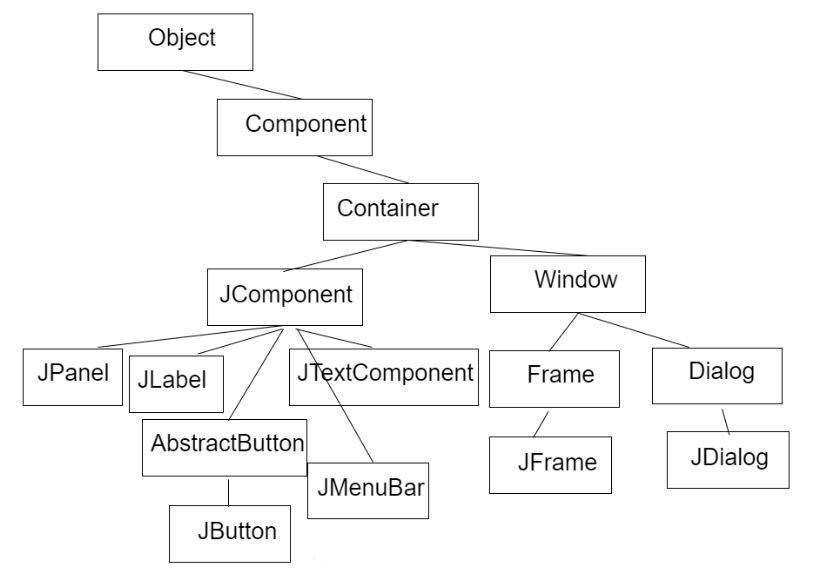
\includegraphics[scale=0.4]{images/Interfacce grafiche/Componenti.png}
    \caption{Gerarchia delle classi di interfaccia grafica}
\end{figure}

\section{SWING}

\dfn{JFrame}{
    Un JFrame è un contenitore che permette di creare una finestra.
    Si possono utilizzare diversi layout.

    La sintassi è:
    \begin{itemize}
        \item \texttt{JFrame frame = new JFrame("Titolo");}
        \item \texttt{frame.setSize(300, 300);}
        \item \texttt{frame.setVisible(true);}
        \item \texttt{JLabel label = new JLabel("Testo");}
        \item \texttt{frame.add(label);}
    \end{itemize}
}

\dfn{Event-driven programming}{
    L'event-driven programming è un paradigma di programmazione in cui il flusso di esecuzione del programma è determinato dagli eventi che avvengono.
    Un evento è un segnale che indica che qualcosa è accaduto.
    Un evento può essere generato da un utente (click del mouse, pressione di un tasto, ...) o da un altro programma.

    \begin{enumerate}
        \item L'applicazione crea gli event-handlers;
        \item L'applicazione registra gli event-handlers\footnote{Questo significa
        che ogni event-handler è legato a un tipo di evento.}.
    \end{enumerate}

}

\begin{figure}[h]
    \centering
    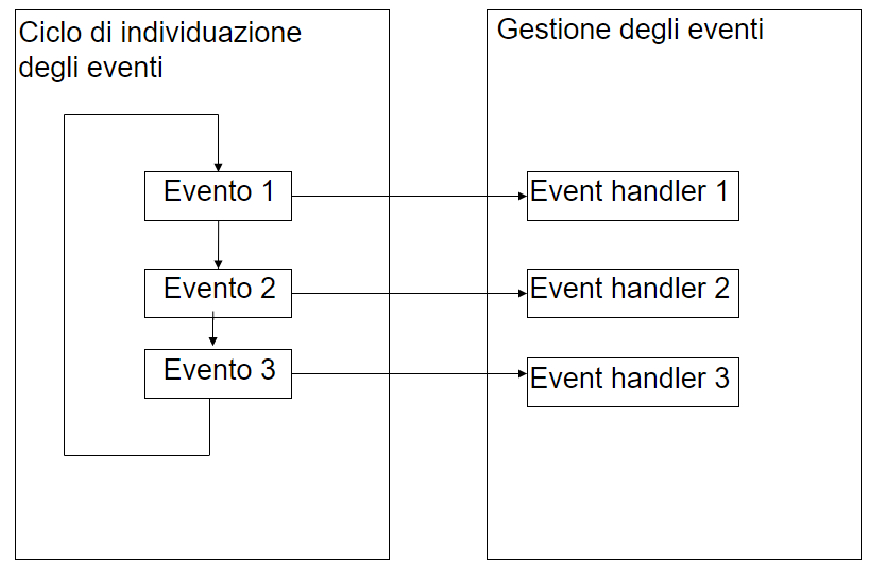
\includegraphics[scale=0.4]{images/Interfacce grafiche/Event driven.png}
    \caption{Eventi}
\end{figure}

\nt{Il ciclo degli eventi è un concetto astratto.}

\dfn{Gestione degli eventi}{
    Gli eventi sono passati da un oggetto a un listener che lo gestisce.
    Il listener deve essere registrato presso la sorgente dell'evento.
    Il passaggio dell'evento causa l'invocazione di un metodo del listener.
}

\cor{Listener}{
    Esistono differenti \texttt{interface}:
    \begin{itemize}
        \item ActionListener: gestisce gli eventi generati da un componente che genera azioni (es. JButton);
        \item MouseListener: gestisce gli eventi generati da un componente che genera azioni del mouse;
        \item MouseMotionListener: gestisce gli eventi generati da un componente che genera azioni del mouse;
        \item WindowListener: gestisce gli eventi generati da un componente che genera azioni della finestra (JFrame).
    \end{itemize}
}

\dfn{Adapters}{
    Gli adapters sono classi che implementano un'interfaccia e forniscono un'implementazione vuota di tutti i metodi.
    Questo permette di implementare solo i metodi che interessano.
}

\nt{Ci possono essere casi con ogni bottone associato al proprio listener. Oppure più bottoni con lo stesso listener.}


\section{Pattern Observe - Observable}

\dfn{Pattern Observe - Observable}{
    Il pattern Observe - Observable è un pattern che serve per rendere più modulare 
    il codice e per permettere la comunicazione tra oggetti. Viene usato anche in altri ambiti,
    ma in questo corso ci occuperemo del suo uso in relazione alla GUI.
}

\nt{In Java esistono gli oggetti \texttt{Observer} e \texttt{Observable} che implementano questo pattern,
tuttavia sono deprecate.
}

\dfn{Observer}{
    L'Observer osserva uno o più oggetti Observable, registrandosi presso di essi.
}

\dfn{Observable}{
    L'Observable è un oggetto che può essere osservato da uno o più Observer.
    Quando l'Observable cambia stato, notifica gli Observer.
}

\nt{La notifica viene effettuata tramite il metodo \texttt{update()}.}

\cor{Metodi di Observer}{
    \begin{itemize}
        \item \texttt{update(Observable o, Object arg)}: viene invocato quando l'Observable cambia stato.
    \end{itemize}
}

\cor{Metodi di Observable}{
    \begin{itemize}
        \item \texttt{addObserver(Observer o)}: aggiunge un Observer;
        \item \texttt{deleteObserver(Observer o)}: rimuove un Observer;
        \item \texttt{notifyObservers()}: notifica tutti gli Observer;
        \item \texttt{notifyObservers(Object arg)}: notifica tutti gli Observer con un argomento;
        \item \texttt{deleteObservers()}: rimuove tutti gli Observer.
    \end{itemize}
}

\begin{figure}[h]
    \centering
    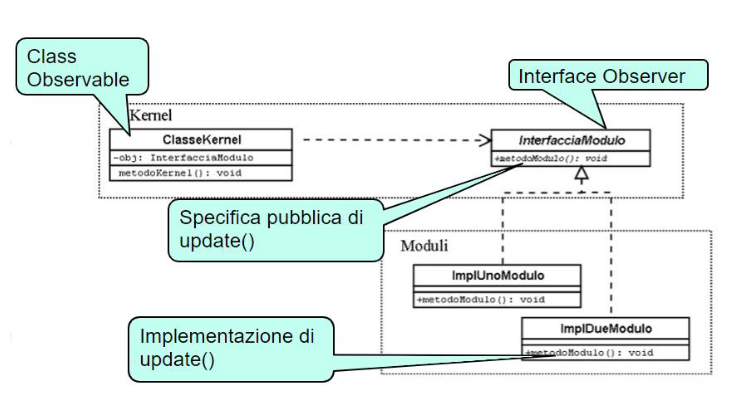
\includegraphics[scale=0.4]{images/Interfacce grafiche/Observer - Observable.png}
    \caption{Pattern Observer - Observable}
\end{figure}

\nt{Le moderne librerie grafiche JavaFX utilizzano questo pattern internamente.}

\section{Pattern MVC}

\dfn{MVC}{
    Un programma si compone di:
    \begin{itemize}
        \item Model: rappresenta i dati e le operazioni che possono essere effettuate su di essi;
        \item View: visualizza i dati e permette l'interazione con l'utente;
        \item Controller: gestisce gli eventi generati dall'utente e aggiorna il model e la view.
    \end{itemize}
}

\nt{Il model è collegato alla view tramite il controller.}

\begin{figure}
    \begin{center}
        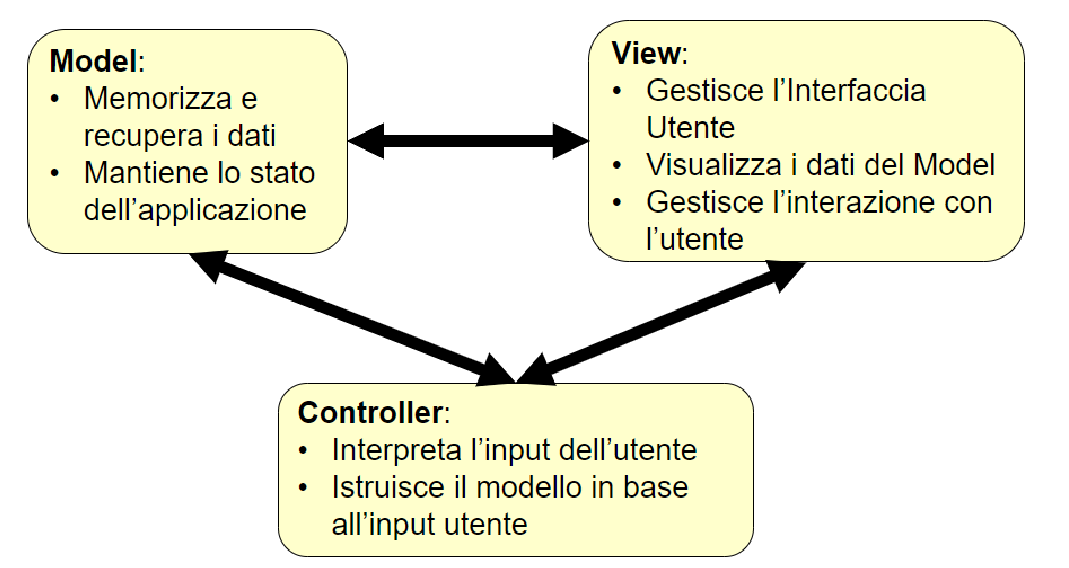
\includegraphics[scale=0.25]{images/Interfacce grafiche/MVC.png}
    \end{center}
    \caption{Pattern MVC}
\end{figure}

\section{XML}

\section{JavaFX}

\dfn{JavaFX}{
    JavaFX è una libreria grafica per lo sviluppo di GUI:
    \begin{itemize}
        \item[$\Rightarrow$] per usarla bisogna aver compreso SWING;
        \item[$\Rightarrow$] separa il contenuto dalla sua visualizzazione tramite fogli
        di stile CSS;
        \item[$\Rightarrow$] permette il binding di properties dei Model;
        \item[$\Rightarrow$] offre classi/interfacce che implementano Observer/Observable;
        \item[$\Rightarrow$] permette di creare interfacce grafiche tramite XML. 
    \end{itemize}
}

\cor{Componenti di JavaFX}{
    \begin{itemize}
        \item \texttt{Stage}: rappresenta una finestra (simile a JFrame);
        \item \texttt{Scene}: rappresenta il contenuto di una finestra.
    \end{itemize}

    La struttura della GUI è gerarchica: nel pannello della scene si inseriscono i
    componenti figli. In uno stage ci può essere una sola scene.
}

\dfn{Form (moduli)}{
    In JavaFX si possono anche creare dei form basati su:
    \begin{itemize}
        \item \texttt{GridPane}: per inserire i componenti grafici in una griglia;
        \item \texttt{Label}: titoli dei campi;
        \item \texttt{TextField}: campi di input;
        \item \texttt{Button}: pulsanti;
        \item \texttt{Text}: testo non modificabile (output). 
    \end{itemize}
}

\dfn{Uso di CSS}{
    Per utilizzare CSS in JavaFX bisogna:
    \begin{itemize}
        \item Creare un file CSS;
        \item Creare un oggetto \texttt{Scene} e associargli il file CSS;
        \item Associare la scena allo stage.
    \end{itemize}
}

\section{JavaFXML}

\dfn{JavaFXML}{
    JavaFXML è un linguaggio di markup basato su XML che permette di creare interfacce grafiche.
    Permette di separare la struttura della GUI dal codice Java.
    Permette di creare interfacce grafiche in modo dichiarativo.
    Permette di utilizzare CSS.
    Permette di utilizzare il pattern MVC.
}

\subsection{Scene Builder}

\dfn{Scene Builder}{
    Scene Builder è un tool che permette di creare interfacce grafiche in modo visuale.
    Permette di creare interfacce grafiche in modo dichiarativo.
}

\subsection{Properties}







